\documentclass{article}

\usepackage[utf8]{inputenc}
\usepackage{amsfonts}
\usepackage{amsmath}
\usepackage{booktabs}
\usepackage{color}
\usepackage{colortbl}
\usepackage{dirtytalk}
\usepackage{graphicx}
\usepackage{hyperref}
\usepackage{listings}
\usepackage[square,sort,comma,numbers]{natbib}
\usepackage{url}
\usepackage{semantic}
\usepackage{tikz}
\usepackage{todonotes}

\lstdefinestyle{Racket}{
  language=Lisp,
  basicstyle=\ttfamily,
  otherkeywords={\#lang,define,match,let,:,->,lambda,struct,define-type,car,cdr},
  identifierstyle=\color{pink!60!blue},
  keywordstyle=\color{blue!50!black},
  stringstyle=\color{green!50!black},
  commentstyle=\color{pink!60!black}
}

\lstdefinestyle{Java}{
  language=Java,
  basicstyle=\ttfamily,
  identifierstyle=\color{orange!40!black},
  keywordstyle=\color{blue!50!black},
  stringstyle=\color{green!50!black},
  commentstyle=\color{blue!50!grey}
}

\lstset{
  style=Racket
}

\usetikzlibrary{shapes.multipart, chains, positioning}
\tikzset{cons/.style n args=2{
    on chain,
    rectangle split,
    rectangle split horizontal,
    rectangle split parts=2,
    draw,
    anchor=center,
    text height=1.5ex,
    node contents={#1\nodepart{two}#2},
    join={by ->}
  }
}

\title{Lecture Notes:\\Functional Programming in Typed Racket}
\author{Florian Biermann \\\small{\texttt{fbie@itu.dk}} \\~}

\date{2016-05-26}

\begin{document}
\maketitle

\section{Hello World in Typed Racket}

\begin{lstlisting}
;; This is a comment!
;; Tell the run-time, which language to use.
#lang typed/racket

;; Now, print something.
(print "Nihao!")
\end{lstlisting}

You must always start your code with a \lstinline{#lang} directive. You can also choose other languages than \lstinline{typed/racket}, such as \lstinline{racket}, \lstinline{plaid} or \lstinline{slides}. For readability, we will omit all \lstinline{#lang} directives in the remaining code examples.

\section{Expressions}

Expressions in Typed Racket are of the form:

\begin{center}
  \lstinline{(f arg1 arg2 ... argn)}
\end{center}

Operators are also just functions:

\begin{center}
  \begin{tabular}{ccc}
    \lstinline{(+ x y)} & $\Rightarrow$ & $x + y$ \\
    \lstinline{(> x y)} & $\Rightarrow$ & $x > y$ \\
    \lstinline{(/ x y)} & $\Rightarrow$ & $\frac{x}{y}$ \\
    \lstinline{(f x y)} & $\Rightarrow$ & $f(x, \, y)$
  \end{tabular}
\end{center}

In Racket this is called an \emph{S-expression}.

\section{Local Bindings}

Local bindings are very similar to local bindings in for instance Java. However, their scope is very explicit:

\begin{lstlisting}
(let ([x (* 2 16)]
      [y (* 3 17)])
    (print (+ x y)))
\end{lstlisting}

Note that, after the final parenthesis that closes the \lstinline{let} expression, you cannot reference \lstinline{x} or \lstinline{y}:

\begin{lstlisting}
(let ([x (* 2 16)]
      [y (* 3 17)])
    (print (+ x y)))
(print x)
\end{lstlisting}

Trying this results in an error:

\begin{verbatim}
; stdin::5873:
;  Type Checker: missing type for top-level identifier;
;  either undefined or missing a type annotation
;   identifier: x
;   in: x
\end{verbatim}

\section{Functions and Types}

We'd like to define a simple function \lstinline{times-two} that multiplies its argument \lstinline{x} by two:

\begin{lstlisting}
(: times-two (-> Number Number))
(define (times-two x)
  (* 2 x))
\end{lstlisting}

There are two things to note here. The first is that there is no return statement in Racket. Instead, a function evaluates to the result of the last expression in its body. The second is that \lstinline{:} denotes a \emph{type annotation}. We have annotated \lstinline{times-two} to be of type $Number \, -> \, Number$.

In a type-expression, the return-type is the last type that occurs. Consider the type \lstinline{(-> A B C)}. The return-type is \lstinline{C} and \lstinline{A} and \lstinline{B} are parameter types. If the type is \lstinline{(-> A B A)}, \lstinline{A} is both parameter and return type. \lstinline{B} is only parameter type.

We could also have written \lstinline{times-two}'s type like this:

\begin{lstlisting}
(define (times-two [x : Number])
  (* 2 x))
\end{lstlisting}

Typed Racket can then infer the correct type of the function. We can ask the REPL\footnote{REPL is short for Read-Eval-Print-Loop.} for the \lstinline{times-two}'s type:

\begin{lstlisting}
> times-two
- : (-> Number Number)
#<procedure:times-two>
\end{lstlisting}

We will often use both notations. The latter notations is in particular used to define the parameter types for \lstinline{struct} constructors.

\section{Conditionals}

This is a well-known function:

\begin{lstlisting}
(: abs (-> Number Number)
(define (abs x)
  (if (< x 0)
      (- x)
      x))
\end{lstlisting}

(Exercise: How else could you have written the type?)

It contains a conditional. Conditionals have the form \lstinline{(if B ET EF)} where \lstinline{B} is a boolean expression, \lstinline{ET} is the expression that is evaluated if \lstinline{B} evaluates to true (\lstinline{#t}), \lstinline{EF} is the expression that is evaluated if \lstinline{B} evaluates to false (\lstinline{#f}).

During the lecture, I told you that the types of \lstinline{ET} and \lstinline{EF} must be the same. This is true in most functional programming languages. However, Typed Racket is a bit special. Look at this example:

\begin{lstlisting}
(define (funny [b : Boolean])
  (if b "True" 54727565))
\end{lstlisting}

Let's check the function's type:

\begin{lstlisting}
> funny
- : (-> Boolean (U Positive-Index String))
#<procedure:funny>
\end{lstlisting}

Instead of raising a type-error, Typed Racket infers from the usage of the conditional, that the return-type of \lstinline{funny} must be the union of the types of both branches. \lstinline{U} stands for set-union, $\bigcup$.

Typed Racket features polymorphic types. Polymorphic types in Typed Racket are very explicit:

\begin{lstlisting}
(: twice (All (A) (-> A (Pairof A A))))
(define (twice a)
  (cons a a))
\end{lstlisting}

\lstinline{cons} is the constructor for the \lstinline{Pairof} type. You can read the type annotation as \say{for all types \lstinline{A}, the type of \lstinline{twice} is such that iff you pass it a value of some type \lstinline{A} it will return a pair of type \lstinline{A} $\times$ \lstinline{A}}.

\section{Immutable State and Recursion}

In purely functional languages, you cannot alter the state of the program. You cannot assign to a variable once it has been defined\footnote{Actually, this is possible in Racket, but using side-effects makes everything much more complicated.}. Consider this simple Java program:

\begin{lstlisting}[style=Java]
public static bool isEven(int n) {
  while (1 < n)
    n = n - 2;
  return n == 0;
}
\end{lstlisting}

The function decrements \lstinline[style=Java]{n} until it is less or equal to one. Then, it check whether \lstinline[style=Java]{n} is equal to zero and returns the value of that check. While this is a very simple way to do it, because recursion in Java is costly, we cannot do it that way in Racket, because there, \lstinline{n} can never be changed. Instead, we have to chose the recursive approach:

\begin{lstlisting}
(: is-even? (-> Integer Boolean))
(define (is-even? n)
  (if (< 1 n)
      (is-even? (- n 2))
      (= n 0)))
\end{lstlisting}

Every time, \lstinline{is-even?} is called with an \lstinline{n} that is greater than 1, it calls itself with \lstinline{(- n 2)}. The result is the same, but this way of thinking enables us to decompose a function into its \emph{cases}!

\section{Pattern Matching}

Pattern matching is a very powerful tool of functional programming. We will use it time and time again to implement functions. Here is a variant of \lstinline{is-even?} that uses pattern matching:

\begin{lstlisting}
(: is-even? (-> Integer Boolean))
(define (is-even? n)
  (match n
    [0 #t]
    [1 #f]
    [_ (is-even? (- n 2))]))
\end{lstlisting}

The principle of the function stays the same: if the value is zero, then it is an even number. If it is one, it is an odd number. In any other case (this is what \lstinline{_} means), the function calls itself recursively and decrements \lstinline{n} by two. The wildcard \lstinline{_} matches any value and it must always come last in the list of patterns, otherwise it will take over all following patterns, too.

By the way, you can use \lstinline{_} anywhere you like if you do not care about the value of something.

\section{Anonymous Functions}

An anonymous function is a function without a name. You can create it and apply it immediately, as in this example:

\begin{lstlisting}
> ((lambda (x) x) 2)
2
\end{lstlisting}

Here, we have defined a lambda expression and applied it to the value \lstinline{2}. We call this function the \emph{identity function}. The line above is equal to $((\lambda\, x\, .\, x)\, 2)$.

\section{The Maybe Type}

The \lstinline{Maybe} type is useful to model the absence of a value without having to explicitly check for null-pointers:

\begin{lstlisting}
(struct None ())
(struct (A) Some ([a : A]))
(define-type (Maybe A) (U None (Some A)))
\end{lstlisting}

The type of \lstinline{Maybe} is the union of two structs and it is polymorphic! \lstinline{A} is just a placeholder, a generic name for a type. It is simlilar, but not equal, to this Java code:

\begin{lstlisting}[style=Java]
  public static abstract class Maybe<A> {}

  public static class None<A> extends Maybe<A> {
    public None() {}
  }

  public static class Some<A> extends Maybe<A> {
    public final A a;
    public Some(A a) {
      this.a = a;
    }
  }
\end{lstlisting}

Now, we can implement a function that performs safe division:

\begin{lstlisting}
(: maybe-divide (-> Number Number (Maybe Number)))
(define (maybe-divide n d)
  (if (= d 0)
      (None)
      (Some (/ n d))))
\end{lstlisting}

We first check whether the divisor \lstinline{d} is zero. If yes, then we cannot divide, so we return \lstinline{None}. Otherwise, we return \lstinline{Some (\ n d)}. This has many benefits. For the first, we do not need to catch any exceptions. Exceptions can go unnoticed when you write your code and then it later becomes a problem in production.

Secondly, the type of \lstinline{maybe-divide} indicates that the computation can go wrong! This is useful information if you are writing an API and want to tell the user of the API that there is a chance for this function to fail. This might be anything from simple arithmetic to HTTP-requests.

We can check whether a \lstinline{Maybe} has a value:

\begin{lstlisting}
(: has-value? (-> (Maybe Any) Boolean))
(define (has-value? m)
  (match m
    [(None) #f]
    [(Some _) #t]))
\end{lstlisting}

We use pattern matching do \emph{decompose} the value of \lstinline{m} in order to see how it has been constructed and what is inside. Note that we do not care what value it contains, so we use \lstinline{_}.

We can use a \emph{higher-order function} -- that is a function that takes another function as an argument -- to only execute a function on a \lstinline{Maybe} if it contains a value:

\begin{lstlisting}
(: maybe-map (All (A B) (-> (-> A B)
                            (Maybe A)
                            (Maybe B))))
(define (maybe-map f m)
  (match m
    [(None) (None)]
    [(Some a) (Some (f a))]))
\end{lstlisting}

\lstinline{maybe-map} is a polymorphic function, because it does not care what the \emph{actual type} of \lstinline{A} and \lstinline{B} is.

\lstinline{f} is of type \lstinline{(-> A B)}. This is the function we want to apply if there is a value present in the maybe. It is important that the types match. Because \lstinline{f} accepts a type \lstinline{A} and returns a type \lstinline{B}, the type of the second parameter to \lstinline{maybe-map} must be of type \lstinline{(Maybe A)} and the return-type must be of type \lstinline{(Maybe B)}.

Now, we can use \lstinline{maybe-map} together with a \emph{lambda expression}:

\begin{lstlisting}
> (maybe-map (lambda ([x : Number]) (* 2 x))
             (maybe-divide 42 23))
- : (U None (Some Number))
(Some 84/23)
\end{lstlisting}

\section{Single-Linked Lists}

Let us try to implement a more interesting data type. Lists are very useful, so let us implement the simplest list possible, a single-linked list. We need an empty list constructor, which we call \lstinline{Nil} and a constructor for adding an element to a list, which we call \lstinline{Cons}:

\begin{lstlisting}
(struct Nil ())
(struct (A) Cons ([head : A] [tail : (LinkedList A)]))
(define-type (LinkedList A) (U Nil (Cons A)))
\end{lstlisting}

Let us instantiate such a list:

\begin{lstlisting}
(Cons 'a
      (Cons 'b
            (Cons 'c
                  (Cons 'd
                        (Cons 'e (Nil))))))
\end{lstlisting}

This is how the list looks like, conceptually:

\begin{center}
  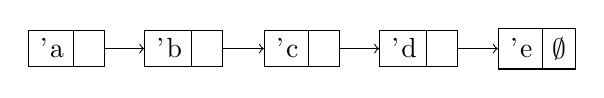
\begin{tikzpicture}[start chain=going right]
    \node (a) [cons={\lstinline{'a}}{}];
    \node (b) [cons={\lstinline{'b}}{}];
    \node (c) [cons={\lstinline{'c}}{}];
    \node (d) [cons={\lstinline{'d}}{}];
    \node (e) [cons={\lstinline{'e}}{$\emptyset$}];
  \end{tikzpicture}
\end{center}

Every list instance contains another, smaller list instance. We call the value of a \lstinline{Cons} cell \lstinline{head} and the remaining list \lstinline{tail}.

Let us see how we can compute the length of a list. We can use pattern-matching:

\begin{lstlisting}
(: list-length (All (A) (-> (LinkedList A) Integer)))
(define (list-length as)
  (match as
    [(Nil) 0]
    [(Cons _ tail) (+ 1 (list-length tail))]))
\end{lstlisting}

There are two cases: either, the list is empty. In this case, the length is zero. Or the list has at least one element. Then, the length is one plus the length of the \lstinline{tail}. Again, note that we do not care about the value of the \lstinline{Cons} cell.

We can easily implement a function to push a new element to the list:

\begin{lstlisting}
(: list-push (All (A) (-> A (LinkedList A)
                            (LinkedList A))))
(define (list-push a as)
  (Cons a as))
\end{lstlisting}

It takes constant time and space, because we re-use the old list. Indeed, many lists can share the same sub-list. For instance, all lists share the empty list \lstinline{Nil}. This is legal, because lists are also immutable\footnote{Sometimes people also call cons-lists a \emph{persistent data structure}.}!

Let us look at more functions on lists. For example, we would like to be able to concatenate two lists. We can again implement this conveniently by pattern-matching.

\begin{lstlisting}
(: list-concat (All (A) (-> (LinkedList A)
                            (LinkedList A)
                            (LinkedList A))))
(define (list-concat lhs rhs)
  (match lhs
    [(Nil) rhs]
    [(Cons head tail) (Cons head
                            (list-concat tail rhs))]))
\end{lstlisting}

Again, we perform case analysis: if the left hand side \lstinline{lhs} is empty, then there is nothing to do and returning whatever is on the right hand side, \lstinline{rhs}, is correct. If however \lstinline{lhs} is not empty, we must add its \lstinline{head} to the new list. How do we construct a new list? By calling \lstinline{list-concat} on its \lstinline{tail}.

Why is this correct? Because either, \lstinline{tail} is \lstinline{Nil}. In this case, \lstinline{concat} will return \lstinline{rhs}. So we have added \lstinline{head} to \lstinline{rhs}. This is, what we wanted. Or, \lstinline{tail} is not empty. Then we add its current \lstinline{head} to whatever is returned by \lstinline{concat} on its \lstinline{tail}. At some point, there is no \lstinline{tail} left, because lists cannot be infinite (computers have finite memory), and we end up again at the base case.

Note, that this takes $O(n)$ time and space, where $n$ is the length of \lstinline{lhs}. We have to look at every element once but we also have to construct $n$ new cells, because we cannot simply replace the empty list at the very end of \lstinline{lhs} by \lstinline{rhs}: lists are also immutable!

The \lstinline{list-remove} function is a nice example to illustrate sub-list sharing. If we know that an element is inside the list, we can ask \lstinline{list-remove} to remove it:

\begin{lstlisting}
> (list-remove
     'c (Cons 'a
              (Cons 'b
                    (Cons 'c
                          (Cons 'd
                                (Cons 'e (Nil)))))))

(Cons 'a (Cons 'b (Cons 'd (Cons 'e #<Nil>))))
\end{lstlisting}

How does it do that? It simply traverses the list and builds new \lstinline{Cons} cells until it encounters \lstinline{'c}. Then it skips \lstinline{'c} and returns the remaining list:

\vspace{1cm}

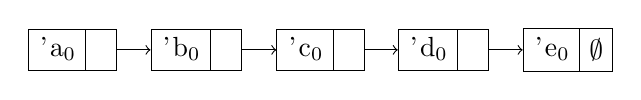
\begin{tikzpicture}[start chain=going right]
  \node (a) [cons={\lstinline{'a}$_0$}{}];
  \node (b) [cons={\lstinline{'b}$_0$}{}];
  \node (c) [cons={\lstinline{'c}$_0$}{}];
  \node (d) [cons={\lstinline{'d}$_0$}{}];
  \node (e) [cons={\lstinline{'e}$_0$}{$\emptyset$}];
\end{tikzpicture}

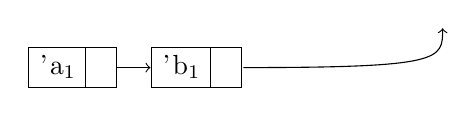
\begin{tikzpicture}[start chain=going right]
  \node (a) [cons={\lstinline{'a}$_1$}{}];
  \node (b) [cons={\lstinline{'b}$_1$}{}];
  \draw [->] (2.17, .0) .. controls (4.7, .0) and (4.7, .1) .. (4.7, .5);
\end{tikzpicture}

\vspace{1cm}

This is the code:

\begin{lstlisting}
(: list-remove (All (A) (-> A (LinkedList A)
                              (LinkedList A))))
(define (list-remove a as)
  (match as
    [(Nil) (Nil)]
    [(Cons head tail)
       (if (eq? head a)
           tail
           (Cons head
           (list-remove a tail)))]))
\end{lstlisting}

\section{Higher-Order Functions on Lists}

Often times, we want to perform the same computation for all values that are stored in a container, such as a list. In functional programming, this can easily be done by using higher-order functions. We have already seen higher order functions for the \lstinline{Maybe} type.

The function that allows us to apply the same function to all elements of a list is typically called \lstinline{map}, because it maps some function to all values that the list contains. If we had no higher-order functions, we would need to write a new function that explicitly traverses the list, every time that we want to modify all list elements. \lstinline{map} makes this unnecessary, because \lstinline{map} rather focuses on the \emph{shape of the data structure} than on whatever function will be executed.

This is our code for \lstinline{map}:

\begin{lstlisting}
(: list-map (All (A B) (-> (-> A B)
                           (LinkedList A)
                           (LinkedList B))))
(define (list-map f as)
  (match as
    [(Nil) (Nil)]
    [(Cons head tail) (Cons (f head)
                            (list-map f tail))]))
\end{lstlisting}

\lstinline{map} does not care what the function \lstinline{f} does, as long as it is of type \lstinline{(-> A B)}. It is perfectly valid for \lstinline{A} and \lstinline{B} to be of the same type. Therefore, we could use a function \lstinline{f} of type \lstinline{(-> Integer Integer)}.

Here is the example from the lecture: a list of students and a function \lstinline{better-grade} that increases the grade of a student by 10\%:

\begin{lstlisting}
(struct Student ([name : String]
                 [grade : Integer]))

(define students
        (Cons (Student "A" 89)
              (Cons (Student "B" 44)
                    (Cons (Student "C" 62) (Nil)))))

(: better-grade (-> Student Student))
(define (better-grade student)
  (Student (Student-name student)
           (+ 10 (Student-grade student))))
\end{lstlisting}

Recall that we can access any field of a struct by calling a function that is named after the pattern \texttt{<struct-name>-<field-name>}. We can now either write a new function that applies \lstinline{better-grade} to every student in a list of students, or we use \lstinline{map} to do so. Here are both variants:

\begin{lstlisting}
(: everyone-better-grade (-> (LinkedList Student)
                             (LinkedList Student)))
(define (everyone-better-grade students)
  (match students
    [(Nil) (Nil)]
    [(Cons student tail)
       (Cons (better-grade student)
             (everyone-better-grade tail))]))
\end{lstlisting}

Note the similarity between \lstinline{everyone-better-grade} and \lstinline{list-map}.

\begin{lstlisting}
> (everyone-better-grade students)
- : (U Nil (Cons Student))
(Cons (Student "A" 99)
      (Cons (Student "B" 54)
            (Cons (Student "C" 72) #<Nil>)))

> (list-map better-grade students)
- : (U Nil (Cons Student))
(Cons (Student "A" 99)
      (Cons (Student "B" 54)
            (Cons (Student "C" 72) #<Nil>)))
\end{lstlisting}

The result is the same, but we only have to write \lstinline{map} once and we can use it on any type of list with any type of function (as long as the functions type is a specialization of the most general type \lstinline{(-> A B)} or $A \, -> \, B$).

If we now want to compute the average of all grades for the course, we need to write a function that first extracts all grades from the students and then adds them together and then finally divides the sum of all grades by the number of students in the course. We could use the following code to get all grades:

\begin{lstlisting}
> (list-map Student-grade students)
- : (U Nil (Cons Integer))
(Cons 89 (Cons 44 (Cons 62 #<Nil>)))
\end{lstlisting}

How do we sum up the resulting grades? We could write a simple sum function, but after we now have learned that we can use higher-order functions to implement re-usable solutions, maybe we can find a way to implement such a function to compute sums. Indeed, such functions exist and one of them is called \lstinline{fold}. It takes a function of type \lstinline{(-> B A B)}, a state parameter of type \lstinline{B} and an input list of type \lstinline{LinkedList A}:

\begin{lstlisting}
(: list-fold (All (A B) (-> (-> B A B)
                            B
                           (LinkedList A) B)))
(define (list-fold f state as)
  (match as
    [(Nil) state]
    [(Cons head tail) (list-fold f
                                 (f state head)
                                 tail)]))
\end{lstlisting}

\lstinline{state} is a parameter that carries the result from the last computation to the next recursive step. We have to initialize it in some way to make sure that we get an answer in case that the input list is empty. Let's try to fold the list of grades with \lstinline{+} (which is of type \lstinline{(-> Integer Integer Integer)} and therefore matches \lstinline{fold}'s type requirement) and see what happens:

\begin{lstlisting}
> (list-fold + 0 (list-map Student-grade students))
- : Integer
195
\end{lstlisting}

We start with zero as the initial state and add every student grade to state. Try, by hand, to take the \lstinline{+} operator, the initial state and the list of grades and to place them in the definition of \lstinline{fold} and see what happens at each step!

Our final function to compute the average of the course could look like this:

\begin{lstlisting}
(: course-average (-> (LinkedList Student) Integer))
(define (course-average students)
  (/ (list-fold + 0 (list-map Student-grade students))
     (list-length students)))
\end{lstlisting}

This is a very concise way of writing this a function, thanks to the higher-order functions we have defined.

Finally, we want to only keep students in the list that have passed the course. Again, we can either write a new function that decomposes the list step by step or we write a higher-order function that removes all elements of a list for which a certain predicate \lstinline{p} holds. Predicates are always of the type \lstinline{(-> A Boolean)}. We call this function \lstinline{filter} and we can define it as follows:

\begin{lstlisting}
(: list-filter (All (A) (-> (-> A Boolean)
                            (LinkedList A)
                            (LinkedList A))))
(define (list-filter p as)
  (match as
    [(Nil) (Nil)]
    [(Cons head tail)
       (if (p head)
           (list-filter p tail)
           (Cons head
                 (list-filter p tail)))]))
\end{lstlisting}

The \lstinline{filter} functions follows the same principle as \lstinline{remove}, but it does not stop after the first element it encounters. It keeps going and calls \lstinline{p} for every element of the list until it reaches the end of the list. We can call it using a lambda expression that returns true if a grade is below 50\%:

\begin{lstlisting}
> (list-filter (lambda ([g : Integer]) (< g 50))
               (list-map Student-grade students))
- : (U Nil (Cons Integer))
(Cons 89 (Cons 62 #<Nil>))
\end{lstlisting}

\end{document}
